\chapter{Tecniche di Machine Learning interpretabile: alberi decisionali}
\label{chap:cap2}
In questo Capitolo, in seguito ad una rapida introduzione generale al \textit{Machine Learning}, viene presentata una delle tecniche di \textit{Machine Learning interpretabile} e cioè gli alberi decisionali.\\
Vengono descritti i concetti fondamentali necessari per costruire le strutture ad albero, i problemi più importanti che si possono incontrare durante questa fase ed i metodi che si utilizzano per risolverli.\\
 In particolare, viene descritto l'algoritmo CART \cite{brei:book}, ovvero l'algoritmo utilizzato in questo lavoro, ed i metodi su cui esso si basa.

\section{Introduzione al Machine Learning}
\label{sec:ml}
Il \textit{Machine Learning, (ML)} è una branca dell’Intelligenza Artificiale e si pone l’obiettivo di far apprendere in modo automatico alle macchine attività svolte da noi esseri umani.\\
Più precisamente, si dice che un programma impara da una certa esperienza $E$ rispetto ad una classe di compiti $T$ ottenendo una \textit{performance P}, se la sua \textit{performance P} nel realizzare i compiti $T$, migliora con l’esperienza $E$ \cite{mitch:book}.\\
In altre parole, se un programma migliora lo svolgere di un \textit{task} rispetto a un’esperienza passata, si dice che ha imparato.\\
Questo avviene tramite l'apprendimento automatico. Esso può essere suddiviso in due importanti categorie: apprendimento supervisionato e apprendimento non supervisionato. 

 Gli algoritmi di apprendimento automatico supervisionato sono sequenze di operazioni che utilizzano i dati di allenamento (\textit{training set}) ricevuti in input per produrre un modello capace di risolvere un problema di classificazione o di regressione su dati di test (\textit{test set}) mai visti in precedenza, con una \textit{performance} che aumenta in funzione della quantità di dati di allenamento ricevuti. In primo luogo, quindi, l'algoritmo lavora su un sottoinsieme del \textit{dataset} chiamato \textit{training set}. Una volta costruito il modello, questo poi viene utilizzato per riconoscere e analizzare dati mai visti (chiamati dati del \textit{test set}).\\
Durante l'apprendimento supervisionato si hanno a disposizione sia i dati di input ($X$, matrice delle $features$ composta dalle variabili indipendenti che usiamo per la predizione), sia i dati di output ($Y$, composto dalle variabili dipendente che vogliamo predire chiamate $labels$). In questo caso si utilizza un algoritmo che apprende la funzione $f$ che dall’input genera l’output: $Y= f(X)$.\\
L’obiettivo è approssimare la funzione in modo che quando si ha un nuovo dato di input l’algoritmo sia in grado di prevedere il valore di output generato per quel dato.\\
I problemi di apprendimento supervisionato possono essere distinti in:
\begin{itemize}
    \item Classificazione: si tratta di un problema discreto, cioè la $label$ è una variabile categorica (si/no, vero/falso, 0/1/2…). Ad esempio, in campo medico, si potrebbe voler determinare in base ai risultati quantitativi di una biopsia se un caso di tumore è benigno o maligno;
    \item Regressione: si tratta di un problema continuo, cioè la $label$ è una variabile numerica. Ad esempio, il prezzo più probabile di una casa che si vuole prevedere sulla base dei metri quadri e della zona di interesse.   
\end{itemize}
Nell’apprendimento non supervisionato, invece, si ha solo la variabile di input $X$ e nessuna variabile di output corrispondente. Pertanto, gli algoritmi di apprendimento non supervisionato cercano di trovare una struttura nel $dataset$.\\
In questo caso i problemi di apprendimento possono essere suddivisi in:
\begin{itemize}
    \item Raggruppamento: anche detto \textit{clustering}, viene utilizzato quando è necessario raggruppare i dati che presentano caratteristiche simili. Per esempio un assicuratore potrebbe voler individuare clienti che corrispondono a profili di rischio simili tra loro, sulla base di caratteristiche quali: l'età, il genere, indicatori dello stato di salute, ecc...;
    \item Associazione: è un problema dove si vogliono scoprire regole che descrivono grandi porzioni di dati; si ha come obiettivo quello di trovare schemi frequenti, associazioni, correlazioni o strutture casuali tra un insieme di oggetti in un \textit{dataset} relazionale. Un'applicazione è quella del \textit{market basket analysis}. Si tratta di analisi di transazioni commerciali che possono produrre informazioni per determinare regole ricorrenti che pongono in relazione l’acquisto di uno o più prodotti con altri. Ad esempio, se un cliente compra il latte qual è la probabilità che compri anche i cereali? Sulla base di queste informazioni si possono progettare azioni promozionali o posizionare gli articoli sugli scaffali;
    \item Riduzione della dimensionalità: è un problema in cui si vuole individuare un numero ridotto di \textit{features} rappresentative delle caratteristiche dei dati all'interno di un grande campione di \textit{features} inizialmente disponibile. Ad esempio, uno psicologo potrebbe utilizzare dati di un campione di studenti delle scuole superiori per costruire un indicatore di abilità linguistica e uno di abilità numerica combinando i voti ricevuti nelle varie materie. Questo consentirebbe la visualizzazione di una pagella come un punto nel piano definito da queste due variabili, invece di trovarsi ad affrontare il problema più complesso di visualizzare contemporaneamente i voti di tutte le materie.
\end{itemize}

In questo lavoro di tesi ho utilizzato un metodo supervisionato  di classificazione: gli alberi decisionali. \MP{Qui direi perchè: sono intepretabili, che é il punto cardine della tesi} Nelle prossime Sezioni, infatti, saranno approfonditi gli aspetti teorici che li riguardano. 

\section{Concetti preliminari: notazione e struttura del dataset}
\label{sec:dataset_class}

In questa Sezione vengono esposti alcuni concetti preliminari che riguardano gli algoritmi di classificazione, necessari per entrare nel merito dei metodi utilizzati per questo lavoro.\\
Il $dataset$ sul quale avviene la fase di addestramento viene chiamato \textit{training set} e il modo più semplice per descriverlo è mediante una matrice $\mathbf{X} \in \mathbb{R}^{n \times \mathbf{m}}$. Le righe della matrice sono i $records$, ovvero gli esempi o le osservazioni e le colonne sono le $features$, cioè le caratteristiche multiple aventi per ogni esempio.\\
Per un algoritmo di classificazione, essendo un metodo di addestramento supervisionato, il $dataset$ è caratterizzato anche dal vettore $Y$ delle $labels$. Ogni $label$, ovvero ogni etichetta, corrisponde ad una classe e sono le variabili target che si vogliono predire (tab. \ref{tab:dataset}).\\

\begin{table}[ht]
    \centering
\begin{tabular}{|c|c|c|c|c|c|}
\hline & feat. $1\left(A_{1}\right)$ & feat. $2\left(A_{2}\right)$ & $\ldots \ldots \ldots$ & feat. $\mathrm{m}\left(A_{m}\right)$ & classe \\
\hline record 1 & & & & & \\
\hline record 2 & & & & & \\
\hline record 3 & & & & & \\
\hline$\ldots \ldots .$ & & & & & \\
\hline$\ldots \ldots$ & & & & & \\
\hline record n & & & & & \\
\hline
\end{tabular}
\caption{Schema della struttura di un generico $dataset$ di apprendimento nel caso in cui si stiano usando algoritmi di classificazione.}
\label{tab:dataset}
\end{table}

La classificazione ha come scopo quello di analizzare i dati di input sviluppando un modello in grado di predire la classe di appartenenza dei  \textit{records} in base alle \textit{features} presenti nei dati. In genere, partendo dall’utilizzo di insiemi esistenti e già classificati, l'algoritmo cerca di identificare alcune regolarità che caratterizzano le varie classi. 

\section{Alberi decisionali: concetti generali}
Gli alberi decisionali sono strutture molto conosciute nell'ambito degli algoritmi supervisionati, in quanto permettono di classificare in modo semplice degli oggetti in un numero finito di classi.

L'utilizzo degli alberi decisionali offre numerosi vantaggi:
\begin{itemize}
    \item sono di facile interpretazione, specie se non sono molto profondi;
    \item ottengono una buona accuratezza su gran parte dei problemi reali di classificazione su dati tabulari;
    \item sono robusti rispetto al rumore e alla ridondanza tra le \textit{features};
    \item possono essere costruiti efficientemente ed essere visualizzati.
\end{itemize}

Gli alberi vengono costruiti suddividendo i $records$ in sottoinsiemi in base alle relazioni che legano le variabili target, che si cercano di prevedere, alle \textit{features} utilizzate come predittori. In particolare, questo permette di costruire un modello rappresentato da un insieme di regole ottenute ponendo una serie di domande (test). Queste sono mirate sui valori delle \textit{features} e tipicamente consistenti in un confronto tra il valore di una data \textit{feature} e una soglia numerica. Ogni volta che si riceve una risposta viene posta la domanda successiva in modo che sia attinente al risultato ottenuto. Il processo viene iterato fino all'ottenimento della classe di ciascun $record$. La serie di domande, e le relative risposte sono organizzate in una struttura ad albero.\\
Fondamentalmente si tratta di una struttura semplice composta da nodi, rami e foglie (anche dette nodi terminali) che si sviluppa a partire dal nodo radice. Ogni nodo corrisponde ad una decisione basata sul confronto di una \textit{feature} con una costante. Essi sono collegati dai rami che identificano i livelli di parentela tra i diversi nodi (il nodo genitore rappresenta una decisione presa a monte rispetto al nodo figlio) e che forniscono gli strumenti per la costruzione di regole necessarie per classificare un oggetto. Infine, i risultati sono identificati dalle foglie. Dato un albero decisionale si possono ottenere predizioni rispetto a nuovi dati semplicemente percorrendo l'albero dalla radice verso le foglie, seguendo di volta in volta il ramo corrispondente al risultato del confronto effettuato in ciascun nodo.

Per fare maggiore chiarezza su come si costruisce un albero decisionale e sulla sua struttura, di seguito viene riportato un semplice esempio.\\
Supponiamo che una compagnia di assicurazioni voglia identificare il legame che lega le classi di rischio, in cui vengono suddivisi i clienti, con la loro età anagrafica e il tipo di vettura posseduto. Lo studio si deve basare su un gruppo di clienti già classificati nella corrispettiva classe.\\ 
Il \textit{training set} $T$ a disposizione è rappresentato in tabella \ref{tab:esempio} e l’insieme delle classi è $\Gamma = \{A, B\}$, in cui $A$ identifica un Alto rischio e $B$ un Basso rischio.

\begin{table}[ht]
    \centering
\begin{tabular}{|c|c|c|c|}
\hline Rid & Età & Tipo di Auto & Rischio \\
\hline 1 & 23 & Berlina & A \\
\hline 2 & 18 & Sportiva & A \\
\hline 3 & 43 & Sportiva & A \\
\hline 4 & 68 & Berlina & B \\
\hline 5 & 32 & Furgone & B \\
\hline6 & 20 & Berlina & A \\
\hline
\end{tabular}
\caption{$Dataset$ d’esempio per classificare clienti di una compagnia di assicurazioni in opportune classi di rischio.}
    \label{tab:esempio}
\end{table}
In figura \ref{fig:esempio} viene riportato un possibile albero decisionale per l'esempio in questione. Si noti come i nodi interni corrispondano a test sulle $features$ e come i nodi foglia vengano etichettati con la classe di maggioranza per la rispettiva foglia.
\begin{figure}
\begin{center}
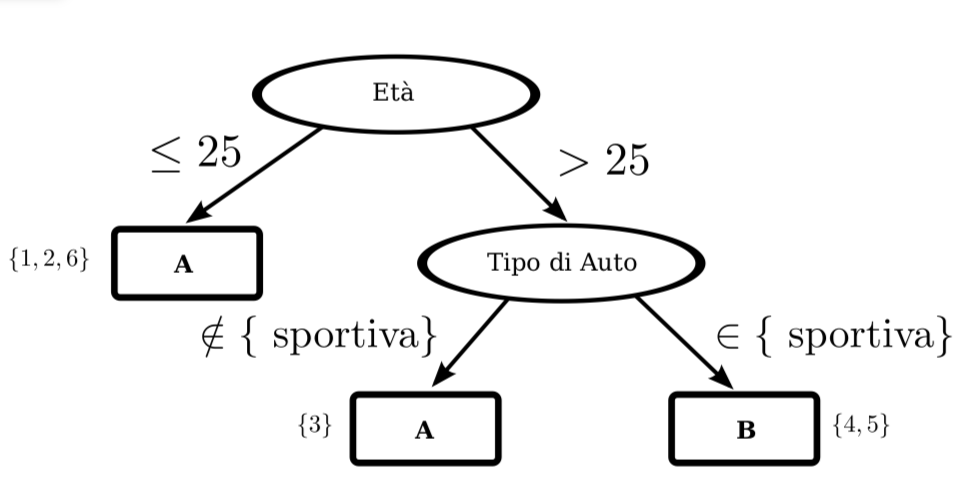
\includegraphics[width=0.5\columnwidth]{images/albero_esempio.png}
\end{center}
\caption{Esempio di albero decisionale per una compagnia di assicurazioni. \MP{Il labeling dell'ultimo nodo mi sembra sbagliato, sono quelli che hanno un'auto sportiva ($\in$ sportiva) che sono ad alto rischio nonostante siano vecchi; $A$ e $B$ nelle foglie andrebbero scambiati.}}
\label{fig:esempio}
\end{figure}

I test sulle \textit{features}, effettuati nei nodi interni, differiscono a seconda del tipo di dati. La suddivisione del $dataset$, dovuta ad esiti diversi nei test, è definita $split$.\\
In questo esempio gli $split$ sono binari, in quanto per ogni nodo si hanno a disposizione due possibilità.

\section{Algoritmo CART}
Esistono in letteratura diversi algoritmi di classificazione che fanno uso degli alberi decisionali. Quello che è stato utilizzato in questo lavoro è l'algoritmo CART.

L'algoritmo CART, \textit{Classification and Regression Trees} \cite{brei:book}, è uno degli algoritmi più conosciuti ed utilizzato per lo sviluppo di alberi decisionali e può lavorare sia come un classificatore che come un regressore.

Uno dei suoi punti di forza è la sua semplicità: esso opera mediante degli $split$ binari (ad ogni nodo corrispondono due soli rami) su una singola variabile in modo ricorsivo, quindi, classificare un campione può richiedere solo pochi semplici passi.\\
Nonostante la sua semplicità, è comunque in grado di ottenere risultati migliori di diversi altri metodi, su $dataset$ complessi, non lineari e composti da molte variabili.\\
Questo è senz'altro un valore aggiunto al fatto che gli alberi decisionali siano di così facile ed intuitiva interpretazione, per questo motivo vengono utilizzati negli ambiti più svariati. Quelle appena discusse sono anche le motivazioni primarie che hanno spinto all'utilizzo di tale metodologia per lo sviluppo di questo progetto di tesi. Trattandosi di un \textit{dataset} non ancora mai sottoposto ad uno studio con metodi di ML, gli alberi decisionali con l'algoritmo CART hanno fornito una prima analisi esplorativa dei dati fornendo già dei buoni risultati \ref{chap:cap4}.

Il metodo CART è molto efficiente anche perché non richiede in ambito applicativo di sperimentare trasformazioni delle variabili indipendenti (logaritmi, radici
quadrate, elevamento a potenza, ecc). Tali trasformazioni, in quanto monotóne, non modificano i risultati a meno che lo $split$ sia basato su combinazioni lineari delle variabili. Questo in genere non succede in un albero convenzionale, dove le \textit{features} vengono valutate indipendentemente in ciascun nodo. Inoltre, esso può utilizzare la stessa variabile in punti differenti dell’albero.\\ 
Il CART è stato creato con lo scopo di trattare dati dotati di una struttura complessa. E' estremamente robusto all’effetto degli \textit{outliers} e può utilizzare congiuntamente variabili di tipo categorico e continue.\\
L'algoritmo CART produce alberi ottimali, utilizzando strumenti sofisticati per stabilirne l'accuratezza (Sez.\ref{sec:metriche}). E, infine, oltre ad essere alla base di altri algoritmi che generano alberi più complessi, esso può essere utilizzato a supporto di altri tipi di modelli.

L'algoritmo si sviluppa in due fasi:
\begin{itemize}
    \item Fase di generazione dell'albero; 
    \item Fase di riduzione della complessità.
\end{itemize}
Vedremo ora quali sono in generale i criteri per la costruzione di alberi decisionali e su quali in particolare il CART si basa.

\section{Criteri per la costruzione di alberi decisionali}
Per costruire una struttura ad albero efficace occorre seguire tre $step$:
\begin{itemize}
    \item Selezionare una regola per lo $split$ per ogni nodo, ciò significa determinare le variabili indipendenti ed i rispettivi valori soglia, che saranno usati per partizionare il \textit{training set};
    \item Determinare quali nodi sono terminali, quindi decidere quando "fermarsi";
    \item Assegnare una classe ad ogni nodo terminale.
\end{itemize}

\section{Regole di Splitting}
Definire le regole di $splitting$ vuol dire identificare, per ogni nodo, una variabile sulla quale effettuare il test sulla base del rispettivo valore soglia utilizzato per il partizionamento del \textit{training set}.\\
Il punto è quello di scegliere in ogni nodo la migliore variabile di $split$, che garantisca la suddivisione dei $records$ presenti nel nodo in sottogruppi il più possibili omogenei al loro interno ed eterogenei tra loro in termini dei valori delle rispettive \textit{labels}.\\
Occorre, quindi, effettuare una sorta di valutazione della bontà degli $split$.\\
A tal proposito gli autori dell'algoritmo CART hanno sviluppato un $framework$ metodologico, introducendo il concetto generico di \textit{impurità}.\\
Intuitivamente, quando dividiamo i dati, vorremmo che la regione corrispondente a ciascun nodo foglia sia "pura", ovvero che la maggior parte dei dati in questa regione provenga dalla stessa classe e quindi che ci sia una classe dominante.

Consideriamo il seguente esempio \cite{split:online} mostrato in figura \ref{fig:impurità}. 
\begin{figure}[ht]
\begin{center}
\includegraphics[width=0.37\columnwidth]{images/impurità1.png}
\includegraphics[width=0.37\columnwidth]{images/impurità2.png}
\end{center}
\caption{Un semplice esempio di $splitting$. La figura a sinistra mostra il primo $split$ (linea blu), mentre quella a destra mostra anche il secondo (linea rossa).}
\label{fig:impurità}
\end{figure}
Qui abbiamo due classi: la classe \textbf{x} e la classe \textbf{o}. Le variabili di input sono la variabile orizzontale e quella verticale. Il primo $split$ viene fatto controllando se la variabile orizzontale è al di sopra o al di sotto di una soglia (la divisione è indicata dalla linea blu).\\
Potremmo considerare questo $split$ una buona divisione perché il lato sinistro è quasi puro in quanto la maggior parte dei punti appartiene alla classe \textbf{x} e solo due punti appartengono alla classe \textbf{o}. Il viceversa vale per il lato destro.\\
Proseguendo ad un livello più in basso nell'albero, vediamo che sono state create altre due divisioni (linee rosse). La regione in alto a sinistra (o il nodo foglia) contiene solo la classe \textbf{x}, così come quella in alto a destra. Invece le regioni in basso a sinistra ed in basso a destra contengono solo la classe \textbf{o}.\\
A questo punto non è necessario effettuare altri $split$ perché tutte le foglie sono pure al $100\%$.


\subsection{La funzione di impurità}
\label{subsec:impurita}
La misura di impurità può essere ricavata a partire dalla cosidetta funzione di impurità $\phi$.\\
Essa misura l'entità della purezza di una regione contenente osservazioni appartenenti a classi possibilmente diverse.

Supponiamo che il numero di classi sia $k$. Quindi la funzione di impurità è definita sul set di \textit{k-tuple} $p_{1},p_{2},...,p_{k}$, che sono le probabilità di ogni osservazione di appartenere ad una certa classe. Vale che $p_{j} \in[0,1]$ $\forall$  $j=1,...,k$ e $\sum_{j} p_{j}=1$.\\
Durante l'addestramento non si conoscono le reali probabilità; si utilizzano, infatti, le percentuali di osservazioni in classe 1, classe 2, classe 3 e così via, in base al set di dati di addestramento.\\
La funzione di impurità può essere pensata come una funzione avente valori tra 0 e 1 che fornisce una misura di quanto le osservazioni siano correttamente distribuite nelle classi.

Si definisce, per un generico nodo $t$, la misura di \textit{impurità} $i(t)$ come segue:
\begin{equation}
i(t)=\phi(p(1 \mid t), p(2 \mid t), \ldots, p(k \mid t))
\label{eq:impurity}
\end{equation}
ove $p(j \mid t)$, con $j=1,...,k$, è la probabilità stimata a posteriori di ottenere la classe $j$ per un'osservazione nel nodo $t$.\\
L’impurità di un nodo è massima quando tutte le classi sono presenti nella stessa proporzione, mentre è minima quando il nodo contiene casi appartenenti ad un’unica classe. La misura di impurità viene usata per decidere quale $split$ fare in un dato nodo, determinando in sostanza in che modo si fa crescere l'albero.

Misure di impurità più comuni sono:
\begin{itemize}
    \item L'indice di eterogeneità di Gini: $\operatorname{Gini}(t)=1-\sum_{j} p_{j}^{2}(t)$
    \item L'entropia: $H(t)=-\sum_{j} p_{j} \log _{2} p_{j}(t)$
    \item Il tasso di errata classificazione: $\operatorname{r}(t)=1-\max \left\{p_{j}(t): 1 \leq j \leq k \right\}$
\end{itemize}


Generalmente, in particolare negli algoritmi che lavorano con $splitting$ binari come CART, viene utilizzato l'indice di Gini.\\
Tale misura può essere interpretata come la stima della probabilità che un’osservazione scelta casualmente nel nodo $t$ sia assegnata alla classe errata.\\
Essa tende a dare luogo a suddivisioni bilanciate dal punto di vista del numero di casi inviati dallo $split$ nei due nodi figli, ovvero tende ad evitare i cosiddetti \textit{small splits}.

\section{Dichiarazione dei nodi terminali}
A questo punto, per completare la costruzione dell'albero è necessario passare per gli ultimi due $step$.\\ 
Bisogna capire, in primo luogo, quando arrestare la "crescita" dell'albero e quindi identificare i nodi terminali. Infine è necessario assegnare una classe ad ogni nodo terminale.  

\subsection{Criteri di arresto}
Nella maggior parte dei casi, se si lasciasse sviluppare un albero fino alle foglie estreme, si avrebbe una struttura molto grande e caratterizzata dal concatenarsi di numerose condizioni. Così facendo, il vantaggio della semplicità interpretativa, caratteristica degli alberi decisionali, verrebbe perso e si andrebbe incontro al problema dell'\textit{overfitting} (approfindito nella Sezione \ref{sec:overfitting}).\\
La dimensione eccessiva sarebbe dovuta al numero di nodi terminali o, equivalentemente, al numero di suddivisioni che essi rappresentano. Per questa ragione, per ovviare al problema, si può decidere di interrompere l’espansione dell’albero sulla base di determinati criteri.\\
Alcuni criteri comuni sono:
\begin{itemize}
    \item  continuare la crescita finché si raggiunge una certa profondità predefinita;
    \item continuare finché il numero di osservazioni in ciascun nodo terminale non superi una certa soglia;
    \item continuare finché tutti i nodi terminali non sono puri, cioè contengono solo una classe \MP{Questo è un po' come non fermarsi però}.
\end{itemize}

Queste soglie vanno decise a priori e influenzano direttamente la dimensione
dell’albero. Per questo motivo, sebbene sia questo il metodo più semplice,
risulta piuttosto inefficiente perché rischia di sfoltire l'albero troppo o troppo poco rispetto al necessario, in base a quanto sia restrittivo il criterio d’arresto.

\subsection{Assegnazione della classe al nodo terminale}
Nella fase di assegnazione di una delle classi ai nodi terminali si possono
presentare tre situazioni diverse:
\begin{itemize}
    \item il nodo contiene solo osservazioni appartenenti alla stessa classe;
    \item il nodo contiene osservazioni appartenenti a classi diverse, ma una di queste presenta una proporzione di osservazioni maggiore delle altre;
    \item Il nodo contiene osservazioni appartenenti a classi diverse e nella stessa proporzione.
\end{itemize}
Nel primo caso l’assegnazione viene effettuata precisamente senza alcun tipo di
indecisione e nel secondo caso il nodo viene assegnato alla classe che presenta più osservazioni. Nell'ultimo caso, invece, si presenta una situazione di massima incertezza, in quanto la probabilità delle classi risulta identica per ciascuna di esse. Pertanto si ricorre ad un tipo di assegnazione
casuale salvo l'intervento del ricercatore che può effettuare un’assegnazione diversa sulla base delle sue conoscenze.

\section{Problema dell'overfitting}
\label{sec:overfitting}
Alla fase di costruzione dell'albero decisionale, per far sì che esso si comporti come un buon classificatore, segue la fase di riduzione della complessità dell'albero. Ma prima di approfondire la descrizione che riguarda questa seconda fase, bisogna introdurre un problema con il quale, quasi sempre, tutti gli algoritmi di ML si confrontano: il problema dell'\textit{overfitting}.

Il metodo di classificazione è un processo che si sviluppa in due fasi: la fase di apprendimento e la fase di predizione.\\ 
Nella fase di apprendimento, il modello viene sviluppato sulla base di dati di allenamento conosciuti, che abbiamo chiamato \textit{training set}.\\
Successivamente, la fase di predizione viene eseguita su un insieme di dati totalmente nuovi per il modello, il cosiddetto \textit{test set}.\\
In pratica, quindi, il modello apprende informazioni, relazioni e collegamenti durante la prima fase e poi applica tutto ciò che ha acquisito su un nuovo insieme di dati per fornire una predizione.\\
Quello che normalmente accade \MP{dipende... se si allena un modello rigido, per es. una regressione lineare, questo non succede} nelle prime prove di addestramento è che il modello porta a delle prestazioni molto buone sul \textit{trainig set} e alquanto scadenti sul \textit{test set}. Vuol dire che il modello 'impara troppo bene' gli schemi dal \textit{training set}, così tanto da non essere poi in grado di generalizzare quanto appreso su un nuovo gruppo di dati.
\MP{Più che 'imparare troppo bene', il modello impara caratteristiche del training set che sono proprie solo del training set e non si applicano altrove. Per esempio nel training set, per puro caso, tutti i fumatori erano pisani. Nella realtà anche persone di altre città fumano con la stessa probabilità e quindi la città di provenienza è pressoché inutile per prevedere se una persona fuma o meno. Ma, specialmente in training set piccoli, correlazioni spurie di questo tipo possono verificarsi abbastanza di frequente.}

Per 'generalizzazione', quindi, si intende l’abilità di una macchina di portare a termine in maniera accurata esempi o compiti nuovi, che non ha mai affrontato, dopo aver fatto esperienza su un insieme di dati di apprendimento \cite{generalizz:online}.\\
Questo problema è noto con il termine \textit{overfitting}, ovvero si tratta di un problema di sovradattamento da parte del modello ai dati \textit{trainig set}. Si verifica quando il modello viene addestrato eccessivamente su un set di dati rumorosi.\\
Pertanto, a causa di questo problema, quando si sviluppa un albero decisionale, è importante capire quando fermarsi. Se un albero crescesse troppo, fino alle foglie più estreme, oltre a perdere la sua importante caratteristica di essere interpretabile, si andrebbe incontro al problema dell'\textit{overfitting}. Questo è evidente se, ad esempio, avessimo un albero con una sola osservazione per foglia, raggiungendo quindi una purezza perfetta in ciascuna foglia sul \textit{training set}. Se si estendesse al massimo un albero, infatti, tale obbiettivo si potrebbe sempre raggiungere per qualunque scelta dei dati di $training$, ma negli ultimi $split$ l'albero non avrebbe imparato alcuna informazione utile dai dati, adattandosi solo alle idiosincrasie del \textit{training set}. Pertanto, risulterebbe probabile che la \textit{performance} predittiva su dati non visti sia molto inferiore, nonostante la predizione nominalmente perfetta in $training$.

Una tecnica per risolvere tale problema per gli alberi decisionali è la tecnica del \textit{pruning}. In breve, essa consiste nell’ottenere da un albero il più piccolo “sottoalbero” che, di fatto, non comprometta l’accuratezza della classificazione. In particolare, nell'algoritmo CART, la tecnica utilizzata è quella del \textit{Cost-Complexity Pruning} che verrà approfondita nella prossima Sezione.

\section{Cost-Complexity Pruning}
\label{sec:pruning}
Per ridurre la complessità dell'albero affinchè possa essere effettivamente utile nel classificare $records$ e nel fornire regole efficaci, è necessario sfoltire la ridondanza dell’albero, ovvero eliminanare i rami meno significativi.

La tecnica che l'algoritmo CART utilizza prende il nome di \textit{Cost-Complexity Pruning}. Consiste nel far sviluppare l'intero albero e poi estarre da esso il più piccolo "sottoalbero". Quest'ultimo porterà a delle migliori previsioni perché vi sono stati "tagliati" i rami corrispondenti a \textit{splitting} eccessivamente specifici sul \textit{training set} e, quindi, superflui. Infatti \textit{pruning} sta proprio per "potatura".\\ 
Questo processo, appunto, non peggiora l'accuratezza delle previsioni, ma bensì, in genere, le migliora, in quanto, poi, il modello sarà capace di classificare efficientemente anche dati totalmente nuovi.

\subsection{Notazione e metodo}
Ora viene introdotta la notazione necessaria per la trattazione della tecnica del \textit{Cost-Complexity Pruning}.\\
Si definiscono:
\begin{itemize}
    \item $T_{max}$ dimensione di massima crescita dell'albero $T$;
    \item $t$ i nodi genitori;
    \item $t'$ i nodi figli, cioè un nodo collegato tramite un percorso al nodo $t$;
    \item $T_{t}$ un ramo dell'albero $T$ con nodo radice $t$.
\end{itemize}
Un metodo di potatura efficiente dovrebbe garantire che la ricerca della sottostruttura ottimale possa essere trattabile computazionalmente.

L'algoritmo del \textit{Cost-Complexity Pruning} è parametrizzato dal parametro $\alpha \in \mathbb{R}$, $\alpha \in[0,1]$, noto come \textit{parametro di complessità}. Questo parametro viene utilizzato per definire la misura \textit{cost-complexity} $R_{\alpha}(T)$ per ogni sottostruttura $T<T_{max}$ come:
\begin{equation}
R_{\alpha}(T)=R(T)+\alpha|\tilde{T}|
\label{eq:costcompl}
\end{equation}
dove $R(T)$ è il tasso di errata classificazione totale dei nodi terminali (definito \ref{subsec:impurita}) e $|\tilde{T}|$ è il numero di nodi terminali (o nodi foglia) che definisce la complessità dell'albero $T$. Infatti, maggiore è il numero di nodi foglia che l'albero contiene, maggiore è la complessità dell'albero perché vi è maggiore flessibilità nel partizionare lo spazio in parti più piccole e quindi maggiori possibilità di adattare i dati di addestramento.\\
Durante la potatura dell'abero bisogna minimizzare la funzione $R_{\alpha}(T)$ e la sottostruttura che alla fine verrà selezionata dipende dal parametro $\alpha$. Infatti, se $\alpha=0$ verrà scelto l'albero più grande perché il termine di complessità viene essenzialmente eliminato. Per $\alpha$ tendente all'infinito, invece, verrà selezionato l'albero di dimensione 1, cioè un singolo nodo radice.\\
Si può dimostrare \cite{split:online} che per ogni $\alpha$ esiste ed è unica una sottostruttura che minimizza $R_{\alpha}(T)$. Inoltre, si può dimostrare anche che le sottostrutture che minimizzano $R_{\alpha}(T)$ al crescere di $\alpha$ sono annidate. Ovvero, il sottoalbero dell'$\alpha$ successivo è compreso in quello precedente e, quindi, vale che $T_{1}>T_{2}>\cdots>t_{1}$, dove i pedici rappresentano il numero progressivo degli $\alpha$. Praticamente, a partire dalle foglie l'algoritmo procede spostandosi verso la radice valutando in ogni nodo la \textit{cost-complexity} al variare di $\alpha$.

Per fare maggiore chiarezza sul metodo di taglio, in primo luogo, è necessario estendere la definizione \ref{eq:costcompl} a un nodo e ad un singolo ramo fuoriuscente dal nodo:
\begin{itemize}
    \item per qualsiasi nodo $t$ appartenente ad una sottostruttura la \ref{eq:costcompl} diventa: $$R_{\alpha}(t)=R(t)+\alpha$$in quanto ci si sta riferendo proprio ad un nodo, in questo caso non c'è il termine di complessità $|\tilde{T}|$ \MP{non è che non ci sia, ma è uguale a $1$};  
    \item per qualsiasi ramo $T_{t}$, invece la \ref{eq:costcompl} diventa: $$R_{\alpha}\left(T_{t}\right)=R\left(T_{t}\right)+\alpha\left|\tilde{T}_{t}\right|$$ in cui il termine $R\left(T_{t}\right)$ è calcolato considerando tutti i nodi terminali che discendono dal nodo $t$ attraverso il ramo $T_{t}$ (Fig. \ref{fig:potatura}).
\end{itemize}
In ogni nodo, facendo variare $\alpha$ tra 0 e 1 in maniera crescente, l'algoritmo confronta il \textit{cost-complexity} calcolato nel nodo $t$ con quello calcolato per il ramo $T_{t}$. Affinchè l'algoritmo decida di non tagliare un ramo, lo $split$ che avviene per mezzo di esso, deve essere efficiente. Questo si verifica quando lo $split$ riduce l'errore sulla classificazione. Pertanto, finchè $R_{\alpha}\left(T_{t}\right)<R_{\alpha}(t)$ il ramo viene tenuto, ma nonappena i due valori si eguagliano esso viene tagliato. Per cui, la condizione di taglio è data da $R_{\alpha}\left(T_{t}\right)=R_{\alpha}(t)$, da cui:
\begin{equation}
\alpha=\frac{R(t)-R\left(T_{t}\right)}{\left|\tilde{T}_{t}\right|-1}
\label{eq:taglio}
\end{equation}
L'algoritmo lavora percorrendo a ritroso l'albero, dalle foglie verso la radice.\\ Inizialmente, quindi, considera tutti i nodi che precedono le foglie e, facendo variare $\alpha$, il primo nodo trovato che soddisfa la condizione \ref{eq:taglio} viene tagliato. A questo punto, l'algoritmo salva in memoria l'$\alpha$ appena ricavato e poi procede al passo successivo considerando l'albero appena ottenuto come albero iniziale. 
\begin{figure}
\begin{center}
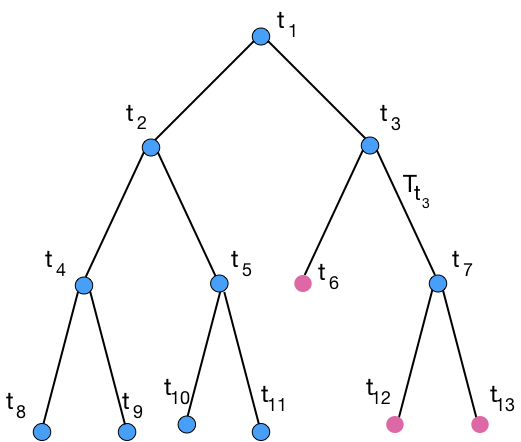
\includegraphics[width=0.37\columnwidth]{images/albero1.png}
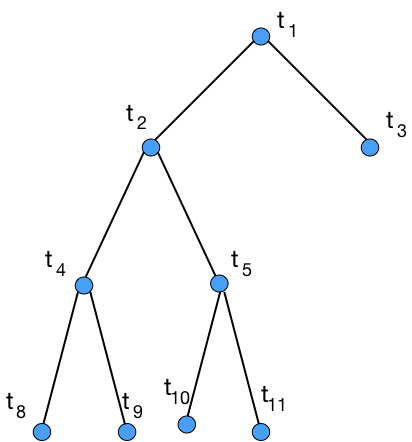
\includegraphics[width=0.30\columnwidth]{images/albero2.png}
\end{center}
\caption{Un semplice schema di una struttura ad albero. I nodi terminali del ramo $T_{t_{3}}$ sono $t_{6}$, $t_{12}$ e $t_{13}$ (a sinistra). In $t_{3}$ si verifica la condizione \ref{eq:taglio}, per cui l'intero ramo $T_{t_{3}}$ viene tagliato (a destra).}
\label{fig:potatura}
\end{figure}

\MP{nella sezione appena conclusa sottolineerei che $\alpha$ è un parametro che l'utente sceglie a mano e che quindi va determinato in base a conoscenze specifiche legate al problema oppure sperimentalmente, tramite validation. Così si transisce in modo naturale alla prossima sezione.}

\section{Training, validation e test sets}
\label{sec:splitdata}
Per identificare i parametri da fornire ai modelli di ML è di uso comune suddividere il \textit{dataset} in tre sottogruppi: \textit{training set, validation set} e \textit{test set}.\\
In questo caso particolare, per effettuare un \textit{pruning} efficiente, dal punto di vista pratico, è necessario identificare il parametro di complessità $\alpha$ al quale corrisponderebbe la miglior sottostruttura dell'albero $T$. Infatti, come spiegato nel paragrafo precedente, ad ogni passo l'algoritmo \textit{Cost-Complexity Pruning} salva in memoria il parametro $\alpha$ che soddisfa la relazione \ref{eq:taglio} con il relativo modello ad albero. Sarà l'utente, in una fase successiva, a scegliere tra questi la miglior sottostruttura, cioè quella per cui si ottiene la miglior accuratezza nella classificazione. Per questo motivo si divide il \textit{dataset} in tre sottogruppi.

Il \textit{training set} è l'insieme di dati con i $records$ e le relative $labels$ e serve al classificatore durante la fasse di allenamento per apprendere gli schemi che possono essere utilizzati successivamente per prevedere le $labels$ dei nuovi dati. In questa fase è importante che non venga effettuata nessuna scelta sul modello.

Il \textit{validation set}, invece, è utile per determinare con quali parametri l'algoritmo di classifcazione avrebbe le migliori prestazioni. Nel caso degli alberi decisionali la fase di validazione è necessaria per scegliere il miglior parametro di complessità $\alpha$.

Una volta ottenuto il miglior classificatore bisogna valutare le sue prestazioni su un set di dati completamente nuovo per lui: il \textit{test set}.

La scelta su come effettuare la divisione del \textit{dataset} è individuale, ma generalmente il \textit{test set} rappresenta circa il $20-30\%$ dei dati. La restante parte del \textit{dataset} viene suddiviso nel seguente modo: circa il $70-80\%$ dei dati rimasti costituirà il \textit{training set} e circa il $20-30\%$ farà parte del \textit{validation set}. 

\begin{figure}
\begin{center}
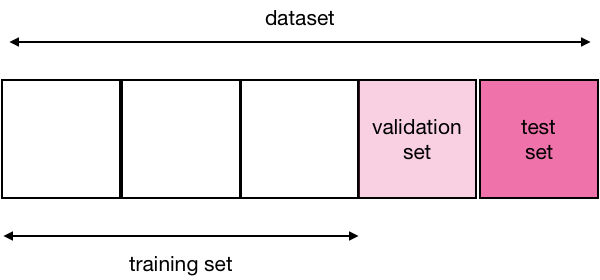
\includegraphics[width=0.6\columnwidth]{images/dataset.png}
\end{center}
\caption{Schema per visualizzare la divisione dei dati nei tre sottogruppi: \textit{training set, validation set} e \textit{test set}.}
\label{fig:dataset}
\end{figure}

\section{Qualità delle previsioni}
\label{sec:metriche}
Per qualsiasi algoritmo di ML, dopo aver ottenuto le previsioni, bisogna valutarne la qualità. Per quantificare la bontà delle \textit{performance} possono essere utilizzate diverse metriche.\\
In questo lavoro, per valutare le prestazioni della classificazione da parte degli alberi decisionali, in primo luogo, è stata utilizzata l'\textit{accuratezza} e, successivamente, altre metriche più adatte \MP{in che senso? Avevamo notato che la sola acciratezza su un dataset sbilanciato dava risultati pessimi, ma poi hai bilanciato il dataset... direi semplicemente altre metriche, che misurano aspetti specifici delle prestazioni di classificazione}, come \textit{precisione, richiamo} ed \textit{F-score (o F-1)}. \MP{Peraltro poi queste metriche vanno spiegate bene, se non qui nel seguito (nel qual caso indicherei che esse sono spiegate nel seguito).}

\subsection{Accuratezza degli alberi decisionali}
Per definire l'accuratezza di un albero decisionale, in primo luogo, introduciamo una notazione. Indichiamo con:
\begin{itemize}
    \item $\bar{n}_{t}$ il numero totale dei $records$ del \textit{test set} che finiscono nel nodo terminale $t$;
    \item $n_{t}$ il numero di $records$ classificati correttamente in $t$.
\end{itemize}
Ad ogni nodo terminale $t$ è possibile associare un'accuratezza $a_{t}$ data dalla frazione dei $records$ classificati correttamente nella data foglia $t$:
\begin{equation}
a_{t}=\frac{n_{t}}{\bar{n}_{t}}
\label{eq:acc_t}
\end{equation}
L’accuratezza nella classificazione associato all’intero albero è data dalla somma delle accuratezze calcolate su tutti i $t$, pesate rispetto alla probabilità che un $record$ possa finire su ciascuna foglia.\\
Se il numero totale di $records$ è $N$ , allora, la probabilità che un certo $record$ finisca nella foglia $t$ è data da $\frac{\bar{n}_{i}}{N}$. Pertanto l'accuratezza $A$ dell'albero risulta:
\begin{equation}
A=\sum_{t} \frac{\bar{n}_{t}}{N} a_{t}
\label{eq:acc}
\end{equation}
La situazione ideale si ha quando $A=1$, in cui il modello è in grado di classificare perfettamente tutti i $records$.\\ 
Questa metrica di solito lavora bene su un set di dati bilanciato, ovvero quando si ha un numero simile di campioni appartenenti a ogni classe.\\
L'accuratezza, però, non è il miglior metodo per valutare le prestazioni di un classificatore.

\subsection{Matrice di confusione: precisione, richiamo e F-score}
\label{subsec:confmatr}
Uno strumento intuitivo per valutare le \textit{performance} di un modello di classificazione è la \textit{matrice di confusione}. Per analizzare le informazioni che essa fornisce bisogna definire le metriche che utilizza e cioè la \textit{precisione}, il \textit{richiamo} e la \textit{F-score (o F-1)}.

Supponiamo di avere due classi: la classe $P$ dei positivi e la classe $N$ dei negativi.\\
Allora, le previsioni ottenute da un modello su un \textit{test set} possono essere definite nei seguenti modi:
\begin{itemize}
    \item \textbf{Veri Positivi} (TP), sono i dati test \MP{realmente} etichettati come $P$ e che il modello ha previsto correttamente come $P$;
    \item \textbf{Falsi Positivi} (FP), sono i dati test etichettati come $N$, ma per i quali il modello ha predetto essere $P$;
    \item \textbf{Falsi Negativi} (FN), sono i dati test appartenenti alla classe $P$, ma per cui il modello ha predetto come $N$;
    \item \textbf{Veri Negativi} (TN), sono i dati test della classe $N$ per i quali il modello ha predetto correttamente collocandoli nella classe $N$.
\end{itemize}
A partire da queste definizioni è possibile introdurre le metriche:
\begin{itemize}
    \item \textbf{Precisione}, $P=\frac{\mathrm{TP}}{T P+F P}$ \MP{il comando mathrm ti permette di far apparire il testo come testo normale dentro ad una espressione matematica; forse puoi provare a usarlo se ti piace il risultato}, è il numero di TP diviso per il numero di classificazioni positive, cioè TP e FP \MP{darei degli esempi: il numero di persone veramente malate su quelle che un dato test ritiene malate}; 
    \item \textbf{Richiamo}, $R=\frac{T P}{T P+F N}$, è il numero di TP diviso per il numero di tutti i $records$ positivi, cioè TP e FN \MP{il numero di persone malate individuate da un test sul totale delle persone veramente malate}; 
    \item \textbf{F-score}, $F_{1}=2 \cdot \frac{P \cdot R}{P+R}$, è una media armonica tra precisione e richiamo \MP{indicherei qui che la media armonica è più vicina al minimo di quanto lo sia la media aritmetica, quindi per ottenere una buona F score bisogna avere sia un buon richiamo che una buona precisione (come dici dopo)}.
\end{itemize}
Un valore vicino a 1 della \textit{F-score} segnala la capacità del modello di classificare correttamente la maggior parte dei dati, ottenendo sia una buona precisione che un buon richiamo (Fig. \ref{fig:prec_ric}). \MP{D'altra parte ottenere un buon richiamo con una pessima precisione è semplice: basta dichiarare tutti malati, riducendo così a zero il numero di falsi negativi al costo di avere molti falsi positivi. Ma il classificatore che ne risulta 
è inutile. Per questo il richiamo da solo non è una buona metrica. Per ragioni analoghe (potrei dichiarare che nessuno è malato, portando i falsi positivi a zero assieme ai veri positivi) la precisione da sola è a sua volta una metrica non buona. Combinandole, la F-score ci garantisce una misura più bilanciata tra questi due aspetti.}

\begin{figure}[ht]
\begin{center}
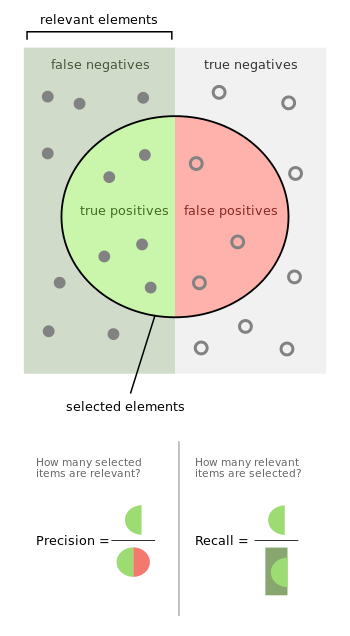
\includegraphics[width=0.4\columnwidth]{images/prec_ric.png}
\end{center}
\caption{Schematizzazione visiva di TP, FP, TN, FN e delle metriche di precisione e richiamo \cite{prec_ric:online}.}
\label{fig:prec_ric}
\end{figure}


Un metodo molto utile per visualizzare queste metriche è la matrice di confusione. Si tratta di uno strumento che mostra la frequenza di errori di classificazione e la corretta classificazione dei dati.\\
Nelle celle di una matrice di confusione sono riportati valori numerici per indicare i vari casi (TP, FP, TN e FN). Pertanto la precisione, il richiamo e, di conseguenza, l' \textit{F-score}, possono essere calcolati direttamente dai valori delle celle di una matrice di confusione.\\
In figura \ref{fig:conf_matr} è riportato uno schema d'esempio di matrice di confusione per un problema di classificazione con due classi.
\begin{figure}[ht]
\begin{center}
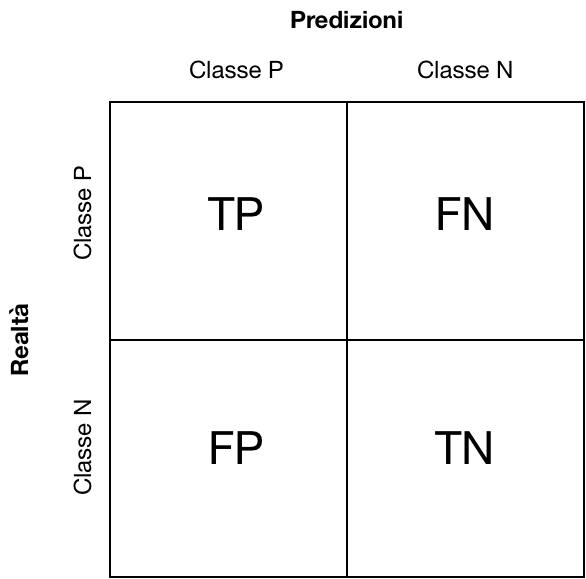
\includegraphics[width=0.5\columnwidth]{images/conf_matr_ok.png}
\end{center}
\caption{Struttura della matrice di confusione nel caso di un problema di classificazione con due classi: $P$ e $N$.}
\label{fig:conf_matr}
\end{figure}
